\section{Periodiska systemet}
\vfill
\begin{figure}[h!]
    \centering
    \label{fig:periodic-table}
    \makebox[\textwidth]{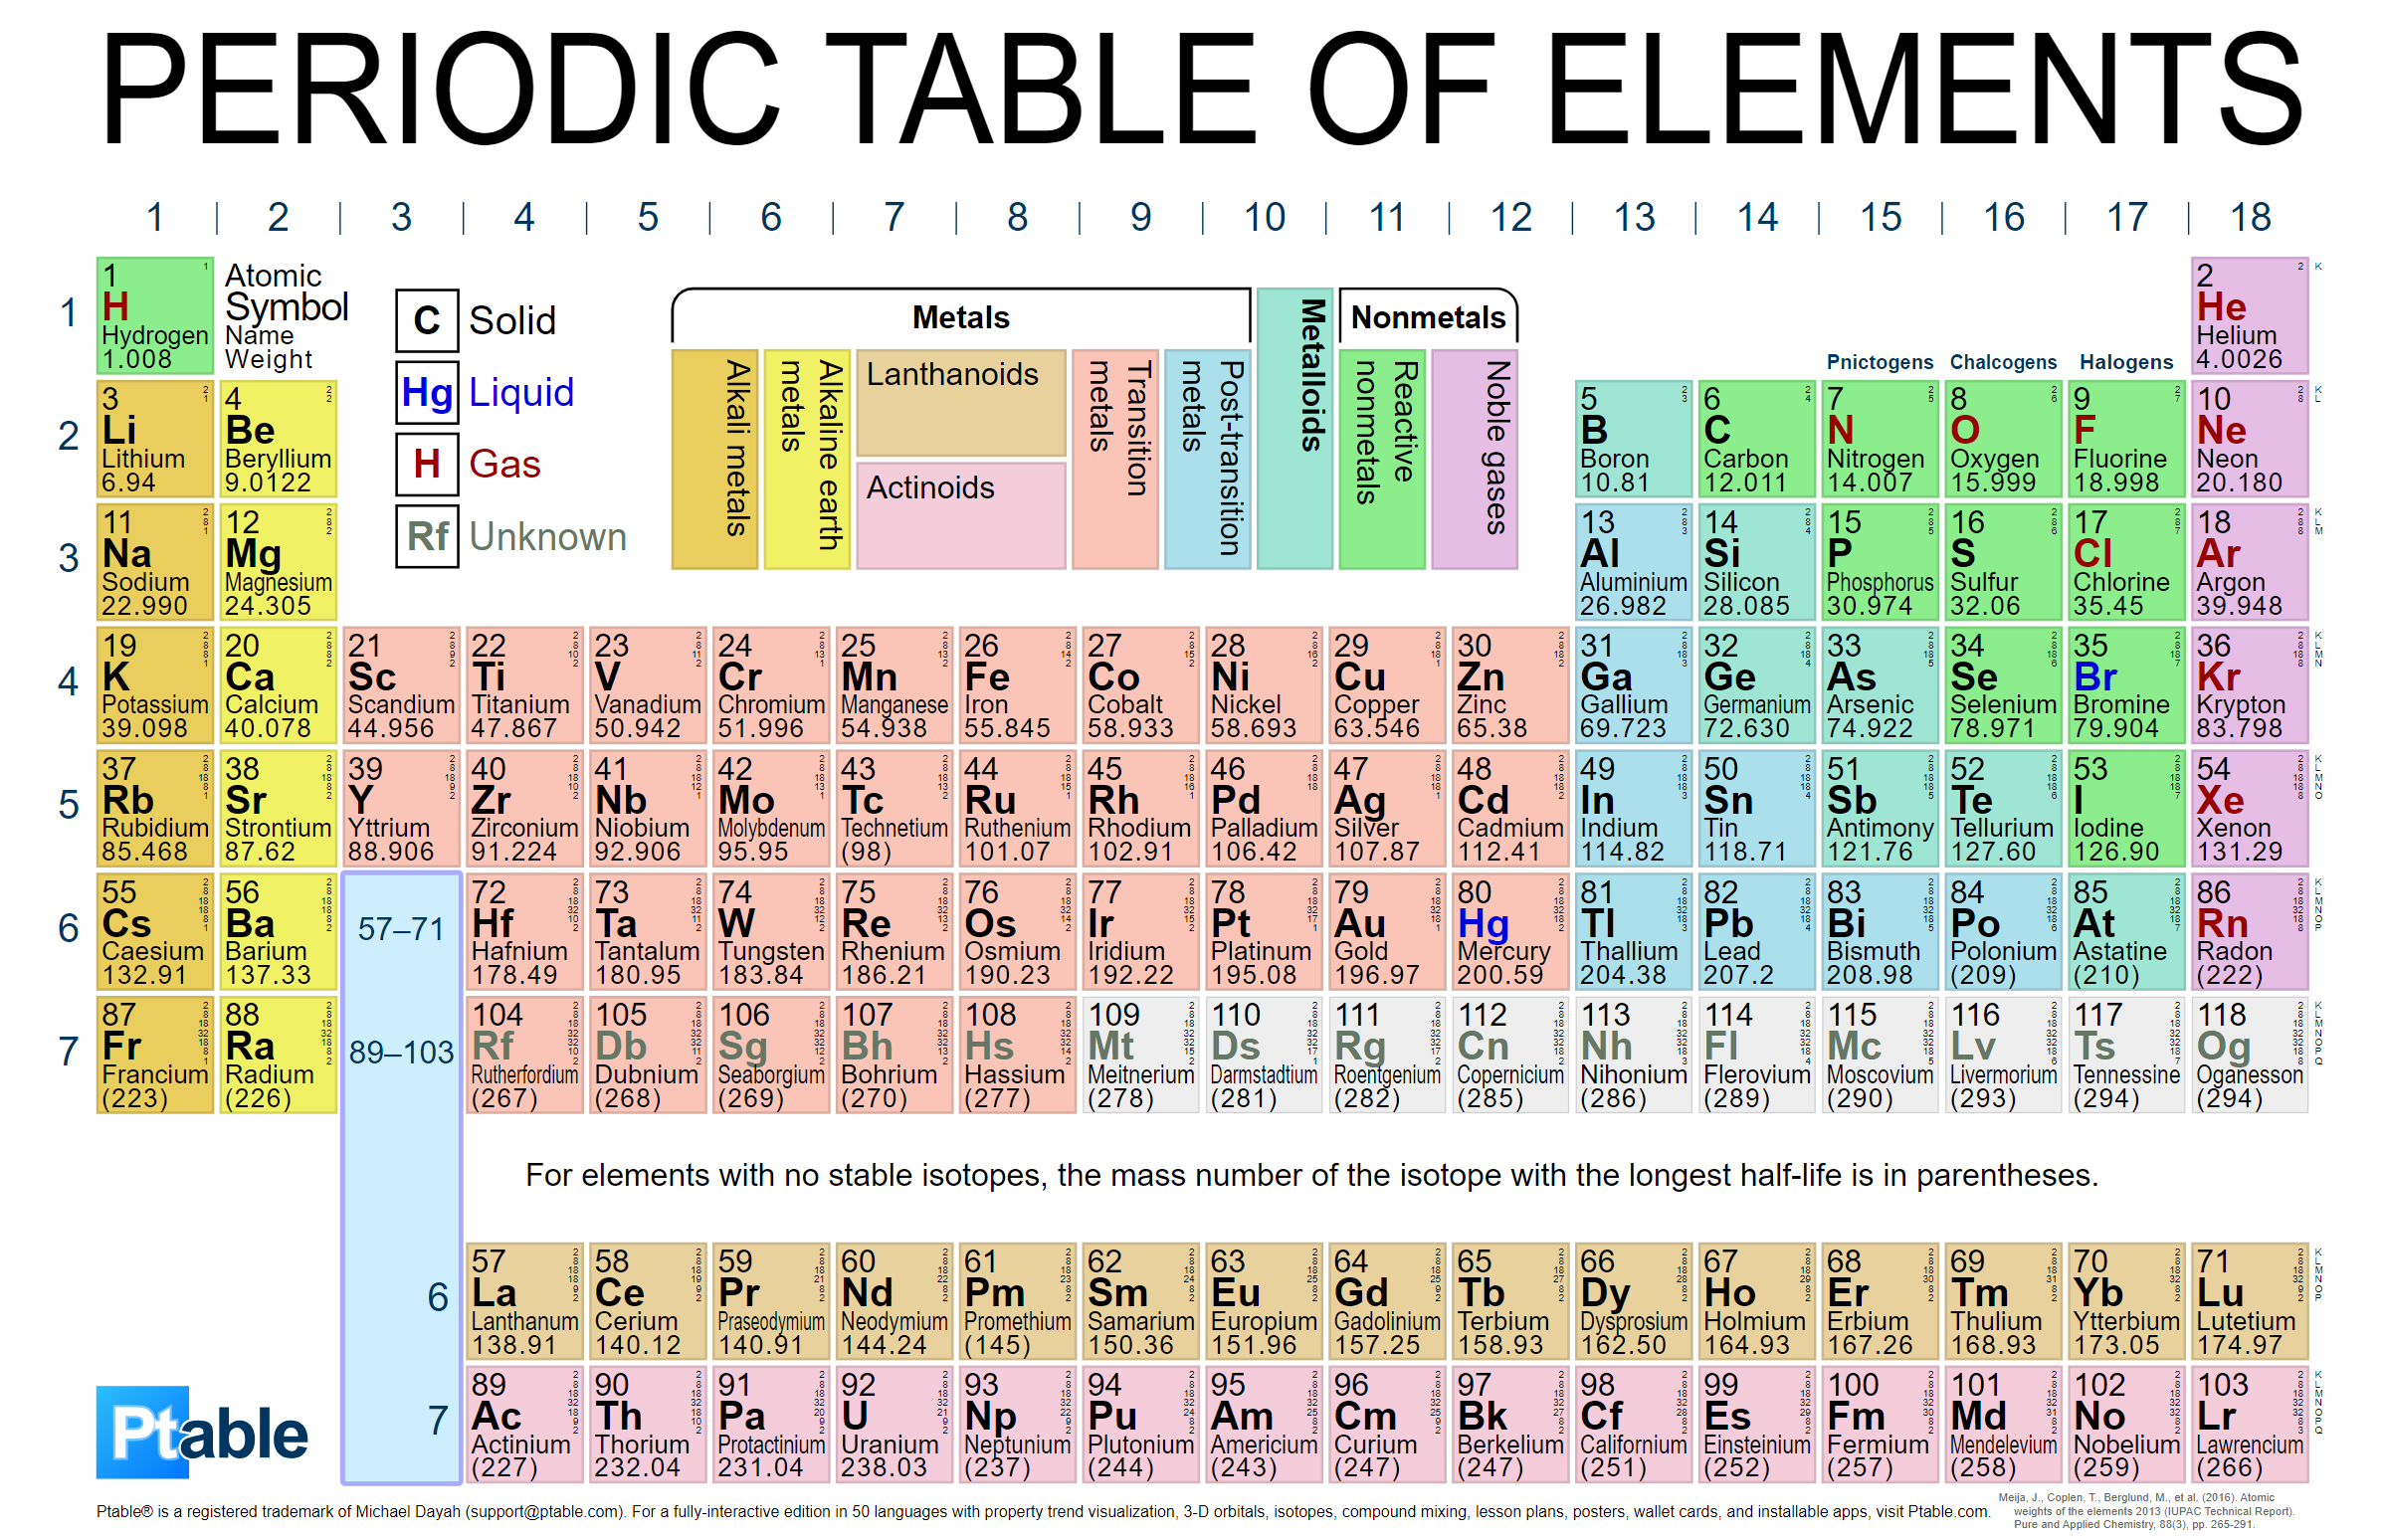
\includegraphics[angle=90,origin=c,width=.629\paperwidth]{img/periodic-table.png}}
    \caption{Periodiska systemet.}
\end{figure}
\vfill
\newpage

\section{Formelsamling}
\centering
\begin{table}[h!]
    \def\arraystretch{1.5}
    \centering
    \caption{Konstanter.}\vspace{5pt}
    \begin{tabular}{c | c | c}
        \textbf{Konstant} & \textbf{Symbol} & \textbf{Värde} \\ \midrule
        Pi & $\pi$ & \num{3.14159265359} \\
        Ljusets hastighet & $c$ & \qty{299792458}{\m\per\s} \\
        Wiens förskjutningskonstant & $b$ & \qty{2.8977719e-3}{\m\kelvin} \\
        Boltzmanns konstant & $k$ & \qty{1.380649e-23}{\joule\per\kelvin} \\
        Plancks konstant & $h$ & \qty{6.62607015e-34}{J\per Hz} \\
        Protonmassa & $m_p$ & \qty{1.673e-27}{\kg} \\
        Neutronmassa & $m_n\approx m_p$ & \qty{1.675e-27}{\kg} \\
        Gravitationskonstanten & $G$ & \qty{6.674e-11}{m^{3}/s^{2}.kg}
    \end{tabular}

\end{table}

\begin{table}[h!]
    \def\arraystretch{1.5}
    \centering
    \caption{Formler.}\vspace{5pt}
    \begin{tabular}{c | c}
        \textbf{Formel} & \textbf{Uttryck} \\ \midrule
        Wiens förskjutningslag & $\displaystyle \lambda_\text{max} = \frac{b}{T}$ \\
        Massa-energiekvivalens & $\displaystyle E = mc^2$\\
        Gravitationslagen & $\displaystyle F_g = G\cdot\frac{m_1m_2}{r^2}$
    \end{tabular}

\end{table}